\documentclass[12pt]{article}

\usepackage{graphicx}% Include figure files
\usepackage{dcolumn}% Align table columns on decimal point

% Use Arial font %
\usepackage{helvet}
\renewcommand{\familydefault}{\sfdefault} 

% Default margins and paper properties %
\usepackage[a4, portrait, margin=0.6in]{geometry}

\begin{document}
	\title{Hypothesis plots summary} % Force line breaks with \\
	\author{1666957, Gustavo Espinal Lugo}
	\date{\today} % It is always \today, today, %  but any date may be explicitly specified

	\maketitle
	%\tableofcontents
	
	\section*{Plots and corresponding metadata}
	Number of data points used: 99999,\\
mean expected W mass: 80.36010913 $[GeV/c^{2}]$,\\
mean hypothesis masses $[GeV/c^{2}]$: [<generator object <genexpr> at 0x7f533a633510>],\\
mass width: 2.07041274 $[GeV/c^{2}]$,\\
chi\_square value of hypothesis fit: 329.3000645043136\\
	Absolute path to figure: /home/physics/phuxdp/Desktop/PX402 Physics Project/WBosonProject/noQED/plots/muPT\_80.36010913\_2.07041274\_between\_31\_and\_131.png\\
	Next lines are the data of the shown histograms (if needed): \\
	All quantities: 	99999, 80.36010913, [ 31.  36.  41.  46.  51.  56.  61.  66.  71.  76.  81.  86.  91.  96.
 101. 106. 111. 116. 121. 126. 131.], 2.07041274, 329.3000645043136\\
	X\_energ\_vls = [30.1, 30.299999999999997, 30.5, 30.700000000000003, 30.9, 31.1, 31.299999999999997, 31.5, 31.700000000000003, 31.9, 32.1, 32.3, 32.5, 32.7, 32.9, 33.1, 33.3, 33.5, 33.7, 33.9, 34.1, 34.3, 34.5, 34.7, 34.9, 35.1, 35.3, 35.5, 35.7, 35.9, 36.1, 36.3, 36.5, 36.7, 36.9, 37.1, 37.3, 37.5, 37.7, 37.9, 38.1, 38.3, 38.5, 38.7, 38.9, 39.1, 39.3, 39.5, 39.7, 39.9, 40.1, 40.3, 40.5, 40.7, 40.9, 41.1, 41.3, 41.5, 41.7, 41.9, 42.1, 42.3, 42.5, 42.7, 42.9, 43.1, 43.3, 43.5, 43.7, 43.9, 44.1, 44.3, 44.5, 44.7, 44.9, 45.1, 45.3, 45.5, 45.7, 45.9, 46.1, 46.300000000000004, 46.5, 46.7, 46.9, 47.1, 47.300000000000004, 47.5, 47.7, 47.9, 48.1, 48.300000000000004, 48.5, 48.7, 48.9, 49.1, 49.300000000000004, 49.5, 49.7, 49.9]\\
	Y\_data\_bin\_cnts = [266.0, 281.0, 301.0, 304.0, 281.0, 321.0, 336.0, 324.0, 300.0, 328.0, 328.0, 325.0, 318.0, 337.0, 328.0, 371.0, 345.0, 331.0, 383.0, 356.0, 327.0, 345.0, 368.0, 354.0, 369.0, 369.0, 367.0, 344.0, 389.0, 342.0, 384.0, 374.0, 371.0, 385.0, 365.0, 370.0, 364.0, 348.0, 351.0, 340.0, 420.0, 408.0, 389.0, 399.0, 403.0, 398.0, 377.0, 376.0, 348.0, 319.0, 320.0, 307.0, 319.0, 305.0, 286.0, 320.0, 272.0, 260.0, 239.0, 235.0, 228.0, 215.0, 216.0, 211.0, 204.0, 180.0, 196.0, 185.0, 158.0, 154.0, 148.0, 127.0, 134.0, 128.0, 120.0, 120.0, 123.0, 101.0, 104.0, 94.0, 110.0, 105.0, 81.0, 79.0, 100.0, 86.0, 75.0, 76.0, 86.0, 83.0, 80.0, 77.0, 65.0, 70.0, 73.0, 61.0, 64.0, 56.0, 57.0, 66.0]\\
	Y\_model\_bin\_cnts = [60.77945327758789, 1.2857933044433594, 6.085181713104248, 3.558061122894287, 1.6192806959152222, 1.9629167318344116, 2.64939546585083, 1.2054215669631958, 13.55706787109375, 2.672044038772583, 4.231561660766602, 114.98712921142578, 1.158971905708313, 3.8883538246154785, 3.0525996685028076, 3.4878652095794678, 1.9948214292526245, 2.6286845207214355, 8.336336135864258, 2.6573493480682373, 25.14351463317871, 2.534775733947754, 1.0967795848846436, 2.5384695529937744, 4.502523899078369, 1.924025297164917, 7.88049840927124, 6.967822551727295, 12.792052268981934, 4.174463272094727, 1.4587275981903076, 11.131487846374512, 1.4413037300109863, 4.7718377113342285, 59.43608856201172, 2.9749960899353027, 219.0475616455078, 2.1233692169189453, 7.402637958526611, 1908.990478515625, 1.5843236446380615, 1.2341128587722778, 174.01522827148438, 1.8120728731155396, 151.42913818359375, 8.514216423034668, 4.172840118408203, 2.9140212535858154, 19.682537078857422, 1.6405428647994995, 3.9315357208251953, 309.38140869140625, 7.394631862640381, 5.369898319244385, 2.2597203254699707, 3.214203357696533, 4.791315078735352, 1190.5732421875, 7.351786136627197, 1.5192288160324097, 6.109335899353027, 4.288990020751953, 18.568132400512695, 1.6339915990829468, 2.035782814025879, 1.3003445863723755, 18.188058853149414, 1.0673106908798218, 5.09853458404541, 34.179039001464844, 26.15125846862793, 53.14067077636719, 2.0191004276275635, 4.089165687561035, 3.968930721282959, 1.1684402227401733, 20.777502059936523, 6.5763468742370605, 3.4533047676086426, 3.826333999633789, 1.0857011079788208, 4.135969161987305, 1.226033091545105, 4.878780364990234, 10.214515686035156, 50.33222579956055, 2.1157166957855225, 21.995885848999023, 15.933954238891602, 3.9041197299957275, 1.8000022172927856, 101.6497573852539, 21.032649993896484, 7.363205909729004, 2.46427845954895, 7.526286602020264, 124.72547149658203, 3.7346036434173584, 1.4995362758636475, 15.372547149658203]\\

    Found optimal massses ($\chi^2$ roots): [74.22745589] $[GeV/c^{2}]$\\
    Uncertainty [GeV/c^2]: 1.4210854715202004e-14\\

	\begin{figure}[tb]
		\centering
		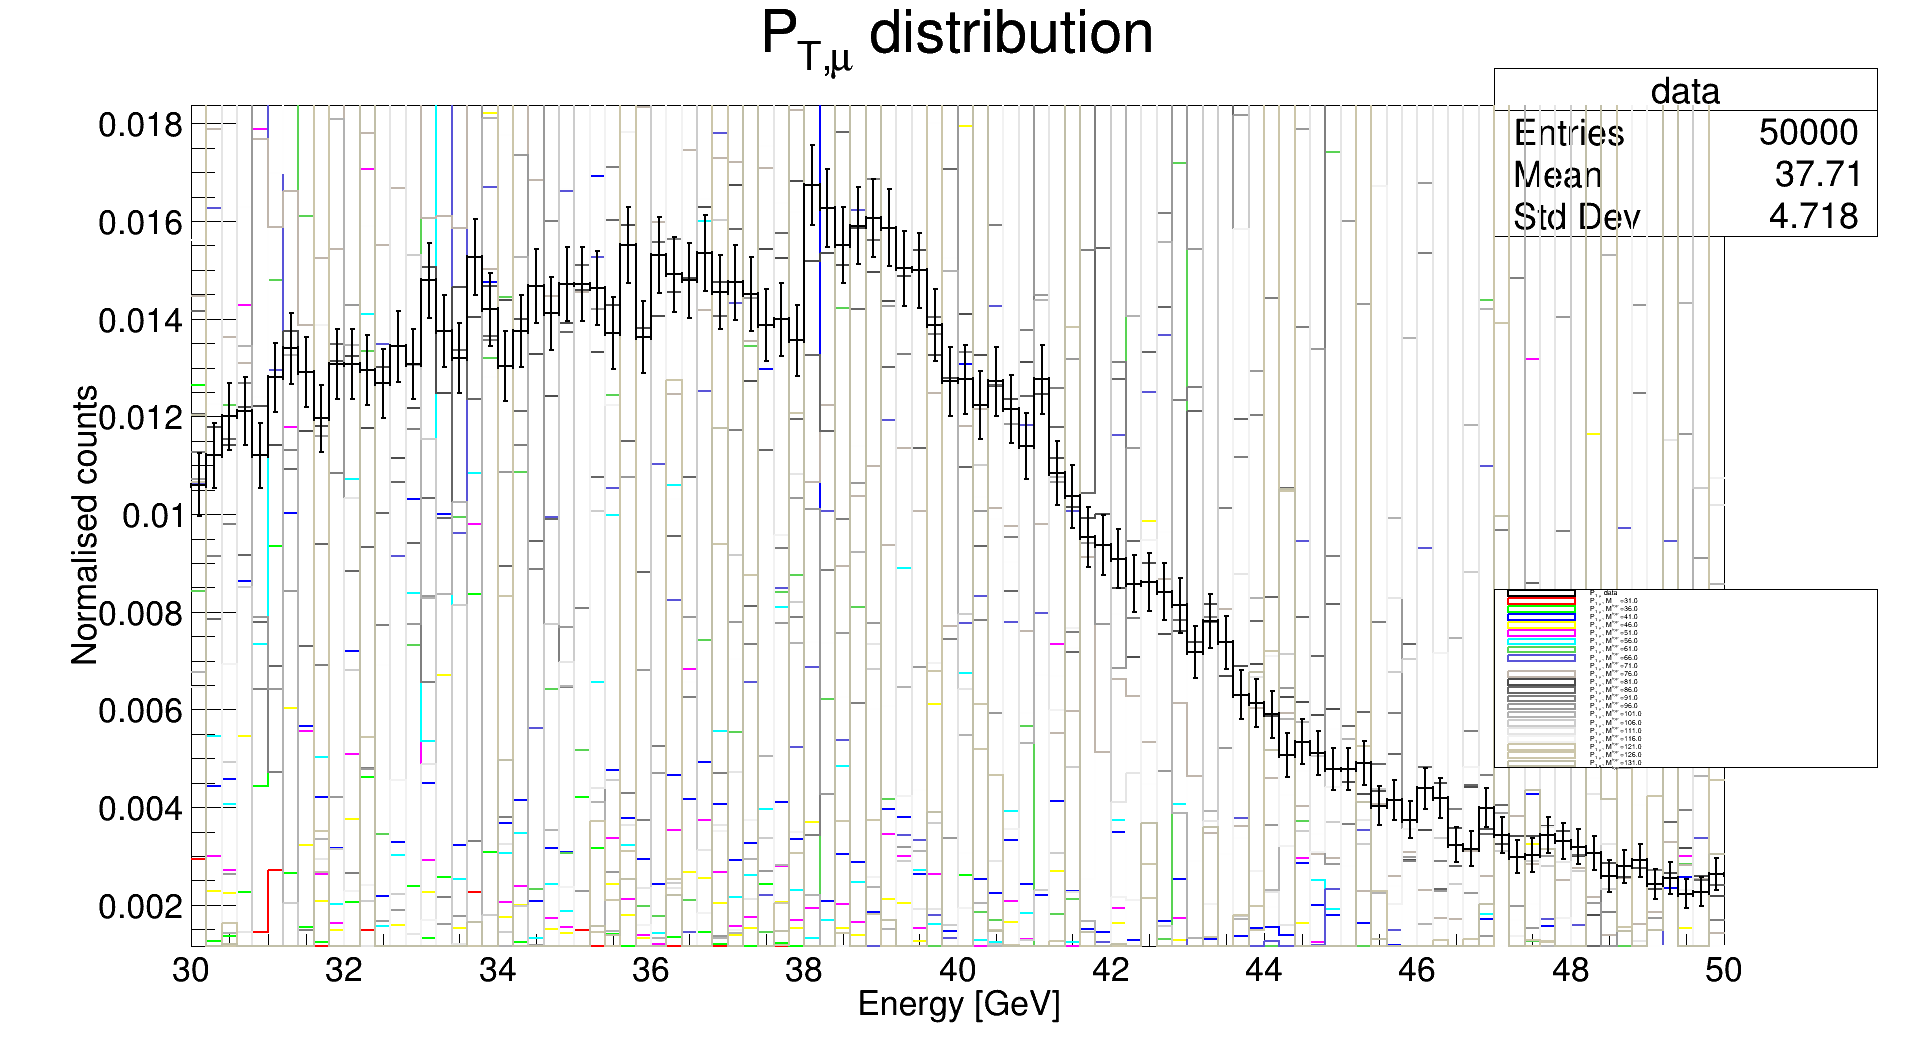
\includegraphics[width=\columnwidth]{/home/physics/phuxdp/Desktop/PX402 Physics Project/WBosonProject/noQED/plots/muPT_80.36010913_2.07041274_between_31_and_131.png}
		\caption{\small Hypothesis masses Number of data points used: 99999,\\
mean expected W mass: 80.36010913 $[GeV/c^{2}]$,\\
mean hypothesis masses $[GeV/c^{2}]$: [<generator object <genexpr> at 0x7f533a633510>],\\
mass width: 2.07041274 $[GeV/c^{2}]$,\\
chi_square value of hypothesis fit: 329.3000645043136. }
		\label{fig: fig_0}
	\end{figure}
    Notes: \\
    1) Using mu\_born\_PT as pseudodata and  Mu\_Pt as model/hypothesis\\
    2) Using full run mode\\
       \begin{figure}[tb]
		\centering
		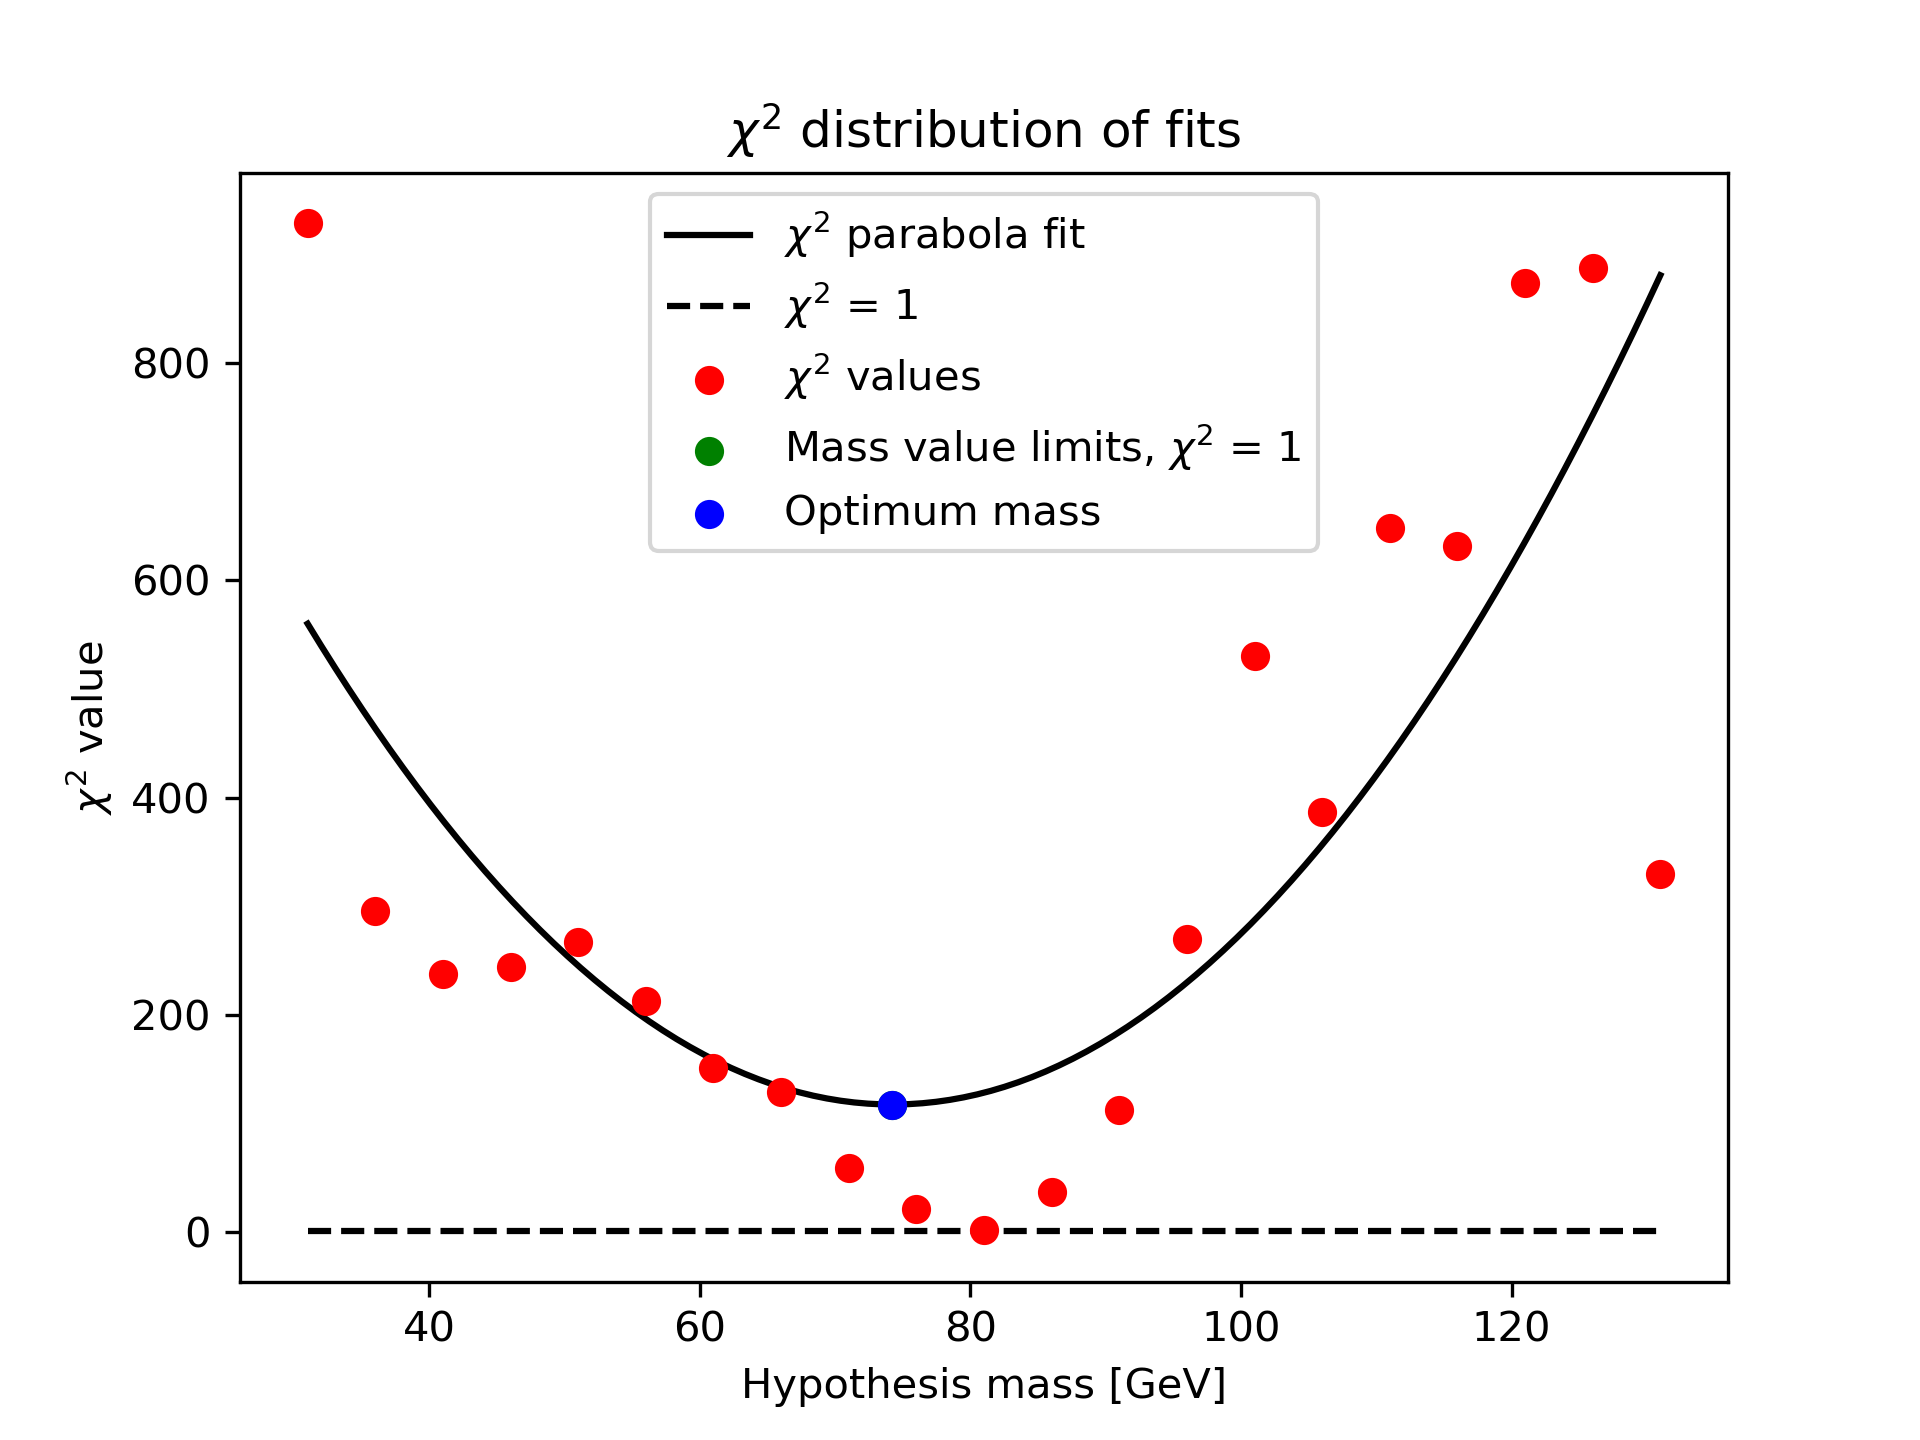
\includegraphics[width=\columnwidth]{/home/physics/phuxdp/Desktop/PX402 Physics Project/WBosonProject/noQED/plots/chi_square_fits_muPT_80.36010913_2.07041274_between_31_and_131.png}
		\caption{\small $\chi^2$ of hypothesis masses. }
		\label{fig: fig_chi_square}
	\end{figure}

    \begin{figure}[tb]
		\centering
		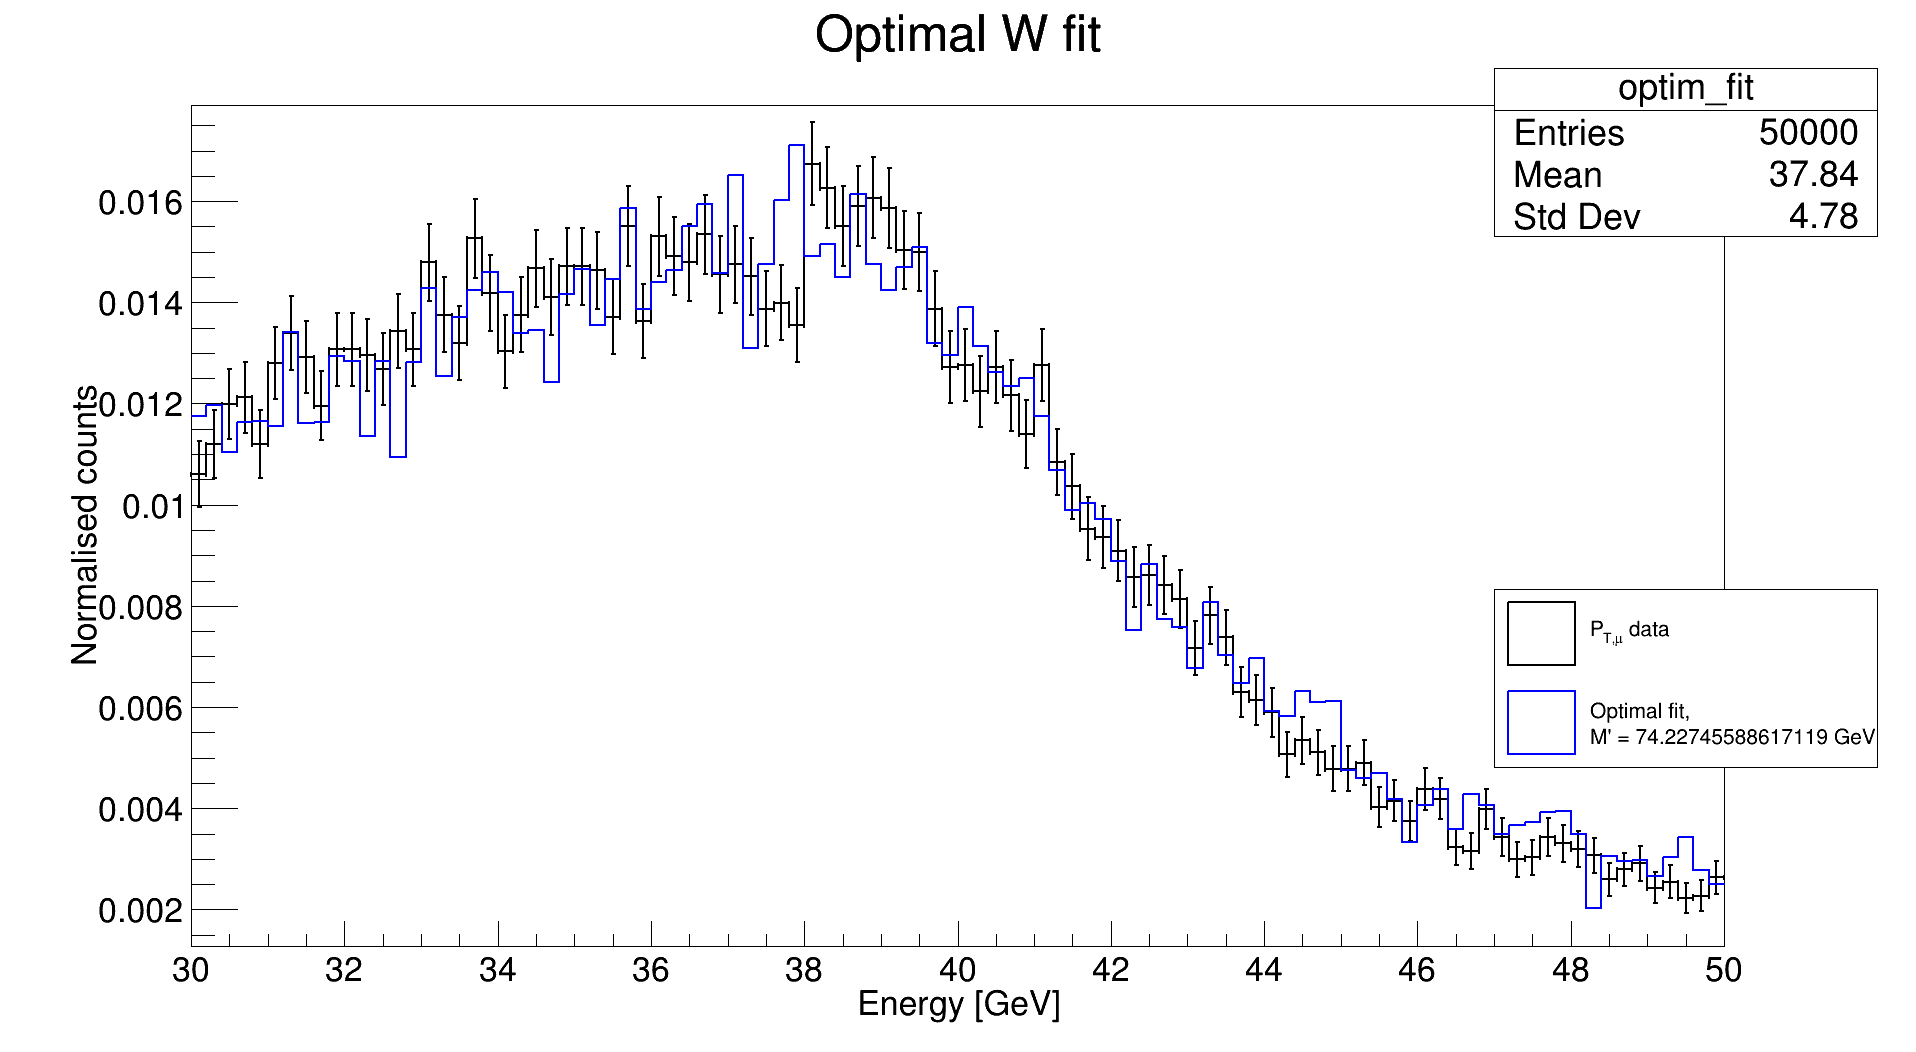
\includegraphics[width=\columnwidth]{/home/physics/phuxdp/Desktop/PX402 Physics Project/WBosonProject/noQED/plots/optimum_muPT_80.36010913_2.07041274_between_31_and_131.png}
		\caption{\small Data and optimum fit with $\chi^2 = 30.652307835646948$. Used the hypothesis mass of 74.22745588617119 $[GeV/c^{2}]$. }
		\label{fig: fig_optim_parms}
	\end{figure}
    
\end{document}